\section{Vorbereitung}
Es sind an einem Universalfilter verschiedenen Filtertypen 2. Ordnung zu Untersuchen. Über die Widerstandsbeschaltung $R_{a},~R_{b},~R_{c},~R_{d},~R_{e}~und~R_{f}$ können bestimmte Filtercharakteristiken, wie Butterworth, Tschebyscheff und Bessel nachgebildet werden.
Mit der Tabelle \cite{Aufgabenstellung} in der Aufgabenstellung sollen bei den Hochpass- und Tiefpassfilter der drei genannten Filtercharakteristiken die Grenzfrequenz $f_{g}$ und die Grundverstärkung $V_{0}$ bestimmt werden.
Bei dem Bandpass ist die Mittenfrequenz $f_{M}$ und die Bandbreite $B$ zu berechnen.
Die Bandsperre wird auf ihre Sperrfrequenz untersucht.



\subsection{Grundverstärkung und Grenzfrequenzen der Hoch- und Tiefpässe}

\subsubsection{Tiefpassfilter}

In der Versuchsbeschreibung \cite{Aufgabenstellung} Kapitel 7: Gleichungen zum Universal-Filter wird die Übertragungsfunktion $H_{TP}$ angegeben mit.\\

\begin{alignat}{2}
H_{TP} (j \omega)&= \frac{U_{TP}}{U_{e}} &= \frac{R_{b} \cdot R_{f}}{R_{a} \cdot R_{c}} \cdot \frac{1}{1+\frac{R_{b} \cdot R_{f}}{R_{c} \cdot R_{e}} \cdot  \left(j \omega \tau \right) + \frac{R_{f}}{R_{d}} \cdot \left ( j \omega \tau \right)^2}~~~~ mit ~\tau = R \cdot C
\end{alignat}

\noindent Durch die Wahl von $R_{b} = R_{c} = R_{f} = R_{0}$ vereinfacht sich die Gleichung zu:

\begin{alignat}{2}
H_{TP} (j \omega) &= \frac{R_{0}}{R_{a}} \cdot \frac{1}{1+\frac{R_{0}}{R_{e}} \cdot  \left(j \omega \tau \right) + \frac{R_{0}}{R_{d}} \cdot \left ( j \omega \tau \right)^2}
\end{alignat}

\noindent Aus der Allgemeinen Gleichung eines Tiefpassfilter 2. Ordnung können so die Parameter $a_{1}, b_{1}~und~V_{0}$ zugewiesen werden. $V_{0}$ ist die maximale Verstärkung bei $\omega -> 0$.

\begin{alignat}{2}
\frac{V_{0}}{1 + a_{1} \cdot j \omega + b_{1} \cdot \left ( j \omega \right)^2} &= \frac{R_{0}}{R_{a}} \cdot \frac{1}{1+\frac{R_{0}}{R_{e}} \cdot  \left(j \omega \tau \right) + \frac{R_{0}}{R_{d}} \cdot \left ( j \omega \tau \right)^2}
\end{alignat}

\begin{alignat}{2}
V_{0} &= \frac{R_{0}}{R_{a}}\\
a_{1} &= \frac{R_{0}}{R_{e}} \cdot \tau\\
b_{1} &= \frac{R_{0}}{R_{d}} \cdot \tau^2
\end{alignat}

\noindent \textbf{Allgemeine Formel zur Bestimmung der Grenzfrequenzen}\\\\

\noindent Der Amplitudengang lautet:

\begin{alignat}{2}
\lvert H_{TP (j \omega)} \rvert = \frac{\lvert V_{0} \rvert}{\sqrt{\left(1 - b_{1} \cdot \omega^2 \right)^2 + a_{1}^2 \cdot \omega^2}}
\end{alignat}

\noindent Mit der Definition $H_{TP (j \omega_{g})} = \lvert H_{TP (j \omega)} \rvert_{max} \cdot \frac{1}{\sqrt{2}}$ und $V_{0} = 1$ (Tabelle \ref{tab:Tiefpaesse_Grundverstaerkung}) kann über einen Koeffizientenvergleich die Grenzfrequenz bestimmt werden.

\begin{alignat}{2}
2 &= \left(1 - b_{1} \cdot \omega^2 \right)^2 + a_{1}^2 \cdot \omega^2\\
0 &= b_{1}^2 \cdot \omega^4 - (2\cdot b_{1} - a_{1}^2) \cdot \omega^2 - 1~~~~~~substituiert~\omega^2 = x\\
0 &= x^2 - \frac{2 \cdot b_{1} - a_{1}^2}{b_{1}^2} \cdot x - \frac{1}{b_{1}^2}
\end{alignat}

\noindent Bestimmen der Möglichen Frequenzen:

\begin{alignat}{2}
x_{1,2} &= -\frac{p}{2} \pm \sqrt{\frac{p}{2}^2 - q}\\
w_{g1} &= +\sqrt{x1}\\
w_{g2} &= -\sqrt{x1}\\
w_{g3} &= +\sqrt{x1}\\
w_{g4} &= -\sqrt{x2}
\end{alignat}

\begin{table}[h]
	\centering
	\begin{tabular}{c|c|c}
		$TP_{Filtercharakteristik}$ & Grundverstärkung $V_{0}$	& Grenzfrequenz $f_{g}$	\\
		\hline
		\hline
		Butterworth	& 1	& 1,5726 kHz	\\
		Tschebyscheff	& 1	& 1,5777 kHz	\\
		Bessel	& 1	& 1,585 kHz 	\\
	\end{tabular}
	\caption{Tiefpassfilter - Grundverstärkung $V_{0}$, Grenzfrequenz $f_{g}$ }
	\label{tab:Tiefpaesse_Grundverstaerkung}
\end{table}

\newpage

\textbf{Bodeplot der TP-Filter Butterworth, Tschebyscheff und Bessel.}

\begin{figure}[h]
\centering
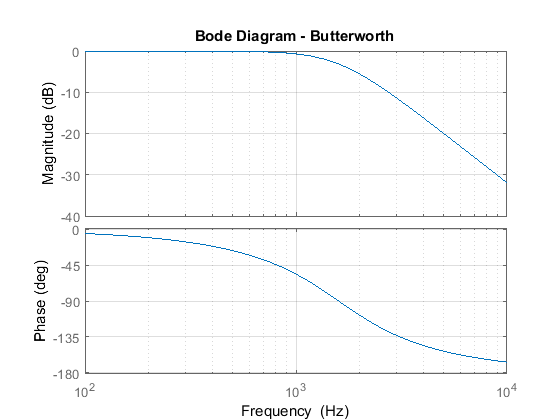
\includegraphics[width=0.7\linewidth]{Bilder/TP_Butterworth}
\caption{}
\label{fig:TP_Butterworth}
\end{figure}

\begin{figure}[h]
\centering
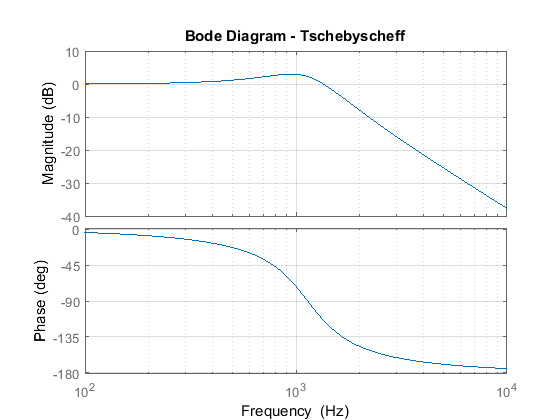
\includegraphics[width=0.7\linewidth]{Bilder/TP_Tschebyscheff}
\caption{}
\label{fig:TP_Tschebyscheff}
\end{figure}

\begin{figure}[h]
\centering
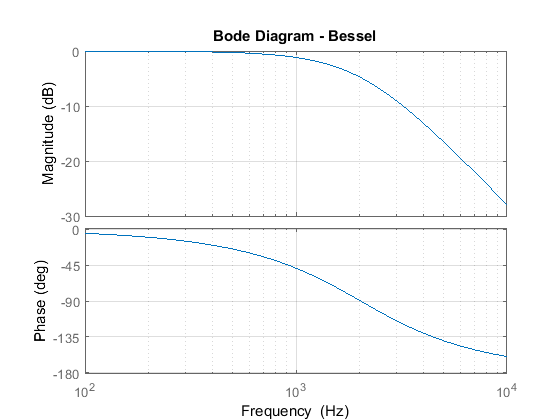
\includegraphics[width=0.7\linewidth]{Bilder/TP_Bessel}
\caption{}
\label{fig:TP_Bessel}
\end{figure}

\newpage


\subsubsection{Hochpassfilter}

In der Versuchsbeschreibung \cite{Aufgabenstellung} Kapitel 7: Gleichungen zum Universal-Filter wird die Übertragungsfunktion $H_{HP}$ angegeben mit.\\

\begin{alignat}{2}
H_{HP} (j \omega)&= \frac{U_{HP}}{U_{e}} &= \frac{R_{b} \cdot R_{d}}{R_{a} \cdot R_{c}} \cdot \frac{ \frac{R_{f} }{R_{d}} \cdot \left( j \omega \tau \right)^2 }{1+\frac{R_{b} \cdot R_{f}}{R_{c} \cdot R_{e}} \cdot  \left(j \omega \tau \right) + \frac{R_{f}}{R_{d}} \cdot \left ( j \omega \tau \right)^2}~~~~ mit ~\tau = R \cdot C
\end{alignat}

\noindent Durch die Wahl von $R_{b} = R_{c} = R_{d} = R_{0}$ vereinfacht sich die Gleichung zu:

\begin{alignat}{2}
H_{HP} (j \omega) &= \frac{R_{0}}{R_{a}} \cdot \frac{ 	\frac{R_{f} }{R_{d}} \cdot \left( j \omega \tau \right)^2 }	 {1+\frac{R_{f} \cdot R_{0}}{R_{0} \cdot R_{e}} \cdot  \left(j \omega \tau \right) + \frac{R_{f}}{R_{0}} \cdot \left ( j \omega \tau \right)^2}
\end{alignat}

\noindent Aus der Allgemeinen Gleichung eines Hochpassfilter 2. Ordnung können so die Parameter $a_{1}, b_{1}~und~V_{0}$ zugewiesen werden. $V_{\infty}$ ist die maximale Verstärkung bei $\omega -> \infty$.

\begin{alignat}{2}
V_{\infty} \cdot \frac{ \frac{1}{b_{1}} \cdot (j \omega)^2}{1 + \frac{a_{1}}{b_{1}} \cdot j \omega + \frac{1}{b_{1}} \cdot \left ( j \omega \right)^2} &= \frac{R_{0}}{R_{a}} \cdot \frac{ \frac{R_{f} }{R_{0}} \cdot \left( j \omega \tau \right)^2  }{1+\frac{R_{f} \cdot R_{0}}{R_{0} \cdot R_{e}} \cdot  \left(j \omega \tau \right) + \frac{R_{0}}{R_{d}} \cdot \left ( j \omega \tau \right)^2}
\end{alignat}

\begin{alignat}{2}
V_{\infty} &= \frac{R_{0}}{R_{a}}\\
b_{1} &= \frac{R_{0}}{R_{f}} \cdot \frac{1}{\tau^2}\\
\frac{a_{1}}{b_{1}} &= \frac{R_{f} \cdot R_{0}}{R_{0} \cdot R_{e}} \cdot \tau\\
a_{1} &= \frac{R_{f} \cdot R_{0}}{R_{0} \cdot R_{e} } \cdot \tau \cdot b_{1}\\
&\Rightarrow \frac{R_{f} \cdot R_{0}}{R_{0} \cdot R_{e} } \cdot \tau \cdot \frac{R_{0}}{R_{f}} \cdot \frac{1}{\tau^2}\\
&\Rightarrow \frac{R_{0}}{R_{e}} \cdot \frac{1}{\tau}
\end{alignat}

\newpage

\noindent \textbf{Allgemeine Formel zur Bestimmung der Grenzfrequenzen}\\\\

\noindent Der Amplitudengang lautet:

\begin{alignat}{2}
\lvert H_{HP (j \omega)} \rvert = \frac{\lvert V_{\infty} \rvert \cdot \left(\frac{1}{b_{1}} \right) \cdot \omega^2}{\sqrt{\left(1 - \left(\frac{1}{b_{1}} \right) \cdot \omega^2 \right)^2 + \left(\frac{a_{1}}{b_{1}} \right) \cdot \omega^2}}
\end{alignat}

\noindent Mit der Definition $H_{HP (j \omega_{g})} = \lvert H_{HP (j \omega)} \rvert_{max} \cdot \frac{1}{\sqrt{2}}$ und $V_{\infty} = 1$ (Tabelle \ref{tab:Tiefpaesse_Grundverstaerkung}) kann die Gleichung nach $\omega_{g}$ aufgelöst werden.

\begin{alignat}{2}
\frac{1}{\sqrt{2}} = \frac{\lvert V_{\infty} \rvert \cdot \left(\frac{1}{b_{1}} \right) \cdot \omega^2}{\sqrt{\left(1 - \left(\frac{1}{b_{1}} \right) \cdot \omega^2 \right)^2 + \left(\frac{a_{1}}{b_{1}} \right) \cdot \omega^2}}\\
\sqrt{2} \cdot \lvert V_{\infty} \rvert \cdot \left(\frac{1}{b_{1}} \right) \cdot \omega^2 = \sqrt{\left(1 - \left(\frac{1}{b_{1}} \right) \cdot \omega^2 \right)^2 + \left(\frac{a_{1}}{b_{1}} \right) \cdot \omega^2}\\
2 \cdot \lvert V_{\infty} \rvert^2 \cdot \left(\frac{1}{b_{1}^2} \right) \cdot \omega^2 = \left(1 - \left(\frac{1}{b_{1}} \right) \cdot \omega^2 \right)^2 + \left(\frac{a_{1}}{b_{1}} \right) \cdot \omega^2\\
0 = \left( \frac{1}{b_{1}^2} - 2 \cdot \lvert V_{\infty} \rvert^2 \cdot \frac{1}{b_{1}^2} \right) \cdot \omega^4 + \left(\frac{a_{1}^2}{b_{1}^2} - 2 \cdot \frac{1}{b_{1}} \right) \cdot \omega^2 + 1
\end{alignat}




\begin{alignat}{2}
0 = x^2 + \frac{a_{1}^2 - 2 \cdot b_{1}}{1 - 2 \cdot \lvert V_{\infty} \rvert^2} \cdot x + \frac{b_{1}^2}{1 - 2 \cdot \lvert V_{\infty} \rvert^2}
\end{alignat}

\noindent Bestimmen der Möglichen Frequenzen:

\begin{alignat}{2}
x_{1,2} &= -\frac{p}{2} \pm \sqrt{\frac{p}{2}^2 - q}\\
w_{g1} &= +\sqrt{x1}\\
w_{g2} &= -\sqrt{x1}\\
w_{g3} &= +\sqrt{x1}\\
w_{g4} &= -\sqrt{x2}
\end{alignat}

\newpage

\begin{table}[h]
	\centering
	\begin{tabular}{c|c|c}
		$HP_{Filtercharakteristik}$ & Grundverstärkung $V_{\infty}$	& Grenzfrequenz $f_{g}$	\\
		\hline
		\hline
		Butterworth	& 1	& 1,6107 kHz	\\
		Tschebyscheff	& 1	& 1,6055 kHz	\\
		Bessel	& 1	& 1,582 kHz 	\\
	\end{tabular}
	\caption{Hochpassfilter - Grundverstärkung $V_{\infty}$, Grenzfrequenz $f_{g}$ }
	\label{tab:Hochpaesse_Grundverstaerkung}
\end{table}

\textbf{Bodeplot der HP-Filter Butterworth, Tschebyscheff und Bessel.}

\begin{figure}[h]
	\centering
	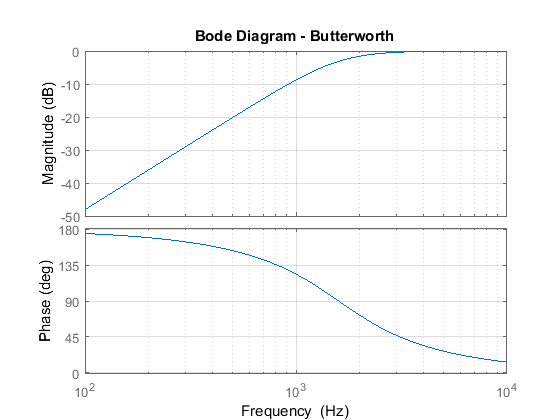
\includegraphics[width=0.7\linewidth]{Bilder/HP_Butterworth}
	\caption{}
	\label{fig:HP_Butterworth}
\end{figure}

\begin{figure}[h]
	\centering
	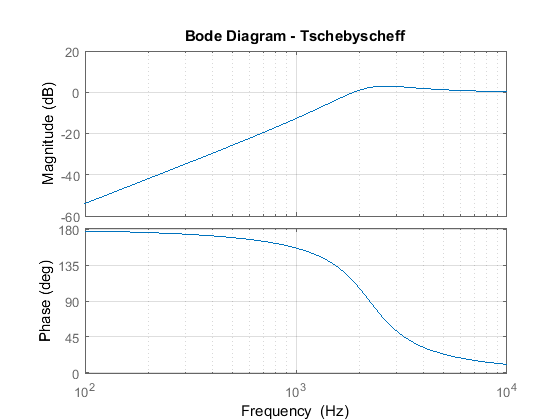
\includegraphics[width=0.7\linewidth]{Bilder/HP_Tschebyscheff}
	\caption{}
	\label{fig:HP_Tschebyscheff}
\end{figure}

\begin{figure}[h]
	\centering
	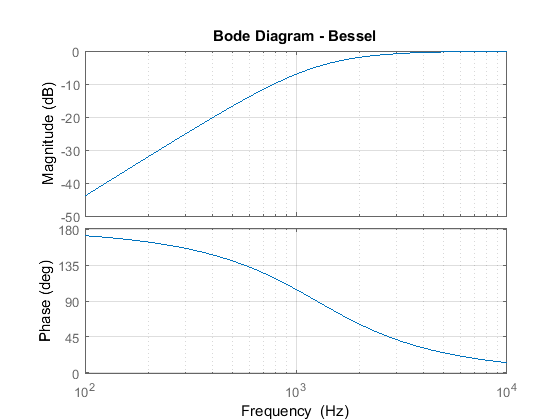
\includegraphics[width=0.7\linewidth]{Bilder/HP_Bessel}
	\caption{}
	\label{fig:HP_Bessel}
\end{figure}

\newpage

\subsubsection{Bandpass}

Die vereinfachte Formel für den Bandpassfilter hergeleitet vom Universalfilter kann der Allgemeinen Übertragungsfunktion eine Bandpassen gleichgesetzt und so die Parameter bestimmt werden.


\begin{alignat}{2}
H_{BP}(j\omega) = V_{max} \cdot \frac{A \cdot j\omega}{1 + A \cdot j \omega + b \cdot (j\omega)^2} \Longleftrightarrow - \frac{R_{0}}{R_{a}} \cdot \frac{\frac{R_{0}}{R_{C}} \cdot (j\omega \tau)}{1 + \frac{R_{0}}{R_{c}} \cdot (j\omega \tau) + (j\omega \tau)^2}
\end{alignat}

Dadurch ergeben sich die nachfolgenden Parameter:

\begin{alignat}{2}
A &= \frac{R_{0}}{R_{c}}\\
b &= \tau^2\\
V_{max} &= - \frac{R_{0}}{R_{a}}
\end{alignat}

\noindent Das Maximum des Bandpassfilter wird erreicht wenn der Imaginärteil des Nenner = 0 ist. Somit entspricht $V_{max}$ dem erreichbaren Maximum. An diesem Punkt befindet sich die Mittenfrequenz $f_{0}$. 

\begin{alignat}{2}
H_{BP}(jw) &= V_{max} \cdot \frac{1}{\frac{1}{j\omega \cdot A} + 1 + \frac{j\omega \cdot b }{A}}\\
&\Rightarrow V_{max} \cdot \frac{1}{1 + j \left(\frac{b}{A}\cdot \omega - \frac{1}{A \cdot \omega} \right)}
\end{alignat}

\begin{alignat}{2}
	0 &= \frac{b}{A} \cdot \omega - \frac{1}{A \cdot \omega}\\
	\frac{1}{A \cdot \omega} &= \frac{b}{A} \cdot \omega\\
	\omega_{0} &= \frac{1}{\sqrt{b}}\\
	f_{0} &= \frac{1}{\tau} \cdot \frac{1}{2 \cdot \pi} = 1,592 kHz\\
	V_{f_{0}} &= 1
\end{alignat}

\noindent Die zwei zu berechnenden Grenzfrequenzen können nach der Definition $H_{BP (j \omega_{g})} = \lvert H_{BP (j \omega)} \rvert_{max} \cdot \frac{1}{\sqrt{2}}$ berechnet werden.


\begin{alignat}{2}
\frac{1}{\sqrt{2}} &= \frac{V_{max} \cdot A \cdot \omega}{\sqrt{\left(1- b\cdot \omega^2 \right)^2 + A^2 \cdot \omega^2}}\\
0 &= x^2 + \frac{A^2 - 2 \cdot b - 2 \cdot A^2 \cdot V_{max}}{b^2} \cdot x + \frac{1}{b^2}
\end{alignat}

\noindent Bestimmen der Möglichen Frequenzen:

\begin{alignat}{2}
x_{1,2} &= -\frac{p}{2} \pm \sqrt{\frac{p}{2}^2 - q}\\
w_{g1} &= +\sqrt{x1}\\
w_{g2} &= -\sqrt{x1}\\
w_{g3} &= +\sqrt{x1}\\
w_{g4} &= -\sqrt{x2}
\end{alignat}

\begin{alignat}{2}
f_{gu} &= 1,4395 kHz\\
f_{go} &= 1,7597 kHz\\
B = f_{go} - f_{gu} &= 320,2 Hz
\end{alignat}

\newpage

\subsubsection{Bandsperre}

Die vereinfachte Formel für den Bandpassfilter hergeleitet vom Universalfilter kann der Allgemeinen Übertragungsfunktion eine Bandpassen gleichgesetzt und so die Parameter bestimmt werden.

\begin{alignat}{2}
H_{BS}(j\omega) = V_{0} \cdot \frac{1 + (j\omega)^2}{1 + A \cdot j \omega + b \cdot (j\omega)^2} \Longleftrightarrow - \frac{R_{0}}{R_{a}} \cdot \frac{1 + (j\omega \tau)^2}{1 + \frac{R_{0}}{R_{c}} \cdot (j\omega \tau) + (j\omega \tau)^2}
\end{alignat}

\noindent Dadurch ergeben sich die nachfolgenden Parameter:

\begin{alignat}{2}
A &= \frac{R_{0}}{R_{c}}\\
b &= \tau^2\\
V_{0} &= - \frac{R_{0}}{R_{a}}
\end{alignat}

\noindent Das Maximum der Bandsperre kann für $\lim\limits_{\omega \to \infty}$ oder $\lim\limits_{\omega \to 0}$ bestimmt werden und strebt gegen 1. Somit kann nach der Definition $H_{BS (j \omega_{g})} = \lvert H_{HP (j \omega)} \rvert_{max} \cdot \frac{1}{\sqrt{2}}$  die Gleichung nach $\omega_{g}$ aufgelöst werden.

\begin{alignat}{2}
\frac{1}{\sqrt{2}} = \frac{\lvert V_{0} \rvert \cdot \lvert 1-  \omega^2 \rvert}{\sqrt{(1- b \cdot \omega^2)^2 + A \cdot \omega^2}}\\
\sqrt{(1- b \cdot \omega^2)^2 + A \cdot \omega^2} = \lvert V_{0} \rvert \cdot \lvert 1-\omega^2 \rvert \cdot \sqrt{2}\\
0 = x^2 + \frac{A^2-2 \cdot b + 2\cdot V_{0}}{b^2} \cdot x + \frac{1-2\cdot V_{0}}{b^2}
\end{alignat}

\noindent Bestimmen der Möglichen Frequenzen:

\begin{alignat}{2}
x_{1,2} &= -\frac{p}{2} \pm \sqrt{\frac{p}{2}^2 - q}\\
w_{g1} &= +\sqrt{x1}\\
w_{g2} &= -\sqrt{x1}\\
w_{g3} &= +\sqrt{x1}\\
w_{g4} &= -\sqrt{x2}
\end{alignat}

\begin{alignat}{2}
f_{gu} &= \\
f_{go} &= \\
B = f_{go} - f_{gu} &= 
\end{alignat}








Werte müssen noch berechnet werden und stammen aus der PSPice simulation.\\

\begin{alignat}{2}
f_{0} &= 1,5922 kHz\\
f_{go} &= 1,76014 kHz\\
f_{gu} &= 1,43911 kHz\\
B &= 321 Hz\\
V_{0,\infty} &= 1
\end{alignat}